\documentclass[conference]{IEEEtran}
\usepackage{cite}
\usepackage{amsmath,amssymb}
\usepackage{graphicx}
\usepackage{booktabs}
\usepackage{multirow}
\usepackage{xcolor}
\usepackage{url}
\usepackage[hidelinks]{hyperref}
\graphicspath{{figures/}}
\newcommand{\inputif}[1]{\IfFileExists{generated/#1}{\input{generated/#1}}{\textit{[table \detokenize{#1} pending]}}}
\newcommand{\figif}[3][\columnwidth]{\IfFileExists{figures/#2}{\includegraphics[width=#1]{#2}}{\fbox{\parbox{#1}{\centering figure \detokenize{#2} pending}}}}
\newcommand{\repo}{\url{https://github.com/maima2024/GenAI-Assignment1}}

\begin{document}

\title{From Universal Autoencoders to Soft Mixtures of Experts and Conditional GANs: A Deployed Study of Image Restoration and Face-to-Sketch Generation}

\author{\IEEEauthorblockN{Umaima Zeeshan}
\IEEEauthorblockA{Roll No.\ 23i-0790 \quad Generative AI, Assignment 1\\
Code: \repo\\ Demo video: \url{https://youtu.be/VIDEO_ID}}}

\maketitle

\begin{abstract}
We design, train, evaluate and deploy four related generative systems. Tasks~1--3 restore $128{\times}128$ Oxford-IIIT Pet images degraded at run time by salt-and-pepper noise, Gaussian blur or rectangular occlusion: (1)~a single universal denoising autoencoder (UDAE) with a genuine spatial bottleneck, (2)~a CNN corruption classifier that hard-routes inputs to one of three independently trained specialist autoencoders (or an identity bypass), and (3)~a jointly fine-tuned soft mixture-of-experts (MoE) whose gate, initialised from the Task-2 classifier, blends all branches. Task~4 is a style-conditioned pix2pix-type conditional GAN that turns FS2K face photographs into sketches in one of three styles through a learned style embedding. Every model is tuned with Optuna, tracked with MLflow, exported to ONNX (with numerical PyTorch/ONNX agreement verified) and served through a FastAPI backend and a React/Tailwind front end orchestrated by Docker Compose. On 36,690 deterministic test inputs, the soft MoE performs best (23.9\,dB / 0.786 SSIM averaged over corruptions, vs.\ 23.2\,dB / 0.705 for the UDAE and 22.8\,dB / 0.724 for hard routing), because its gate learns, without severity labels, to blend the identity branch with the matching expert according to corruption strength. The classifier reaches 99.7\% accuracy, and the cGAN reaches 0.55 SSIM on the FS2K test set, producing clearly style-dependent sketches. We report per-corruption and per-severity results, oracle vs.\ predicted routing, gate behaviour and failure cases.
\end{abstract}

\begin{IEEEkeywords}
denoising autoencoder, mixture of experts, image restoration, conditional GAN, pix2pix, Optuna, ONNX, MLOps
\end{IEEEkeywords}

%=====================================================================
\section{Introduction}
Real images are rarely degraded in a single, known way. A restoration system therefore has to decide \emph{how much} it should specialise: one network can be asked to undo every degradation, a router can pick a dedicated expert, or the experts can be blended softly. Tasks~1--3 of this assignment study exactly this spectrum on a shared data split and a shared deterministic test manifest, so that the three designs are directly comparable. Task~4 moves from restoration to paired image-to-image generation with a conditional GAN, where the conditioning signal (a sketch style) must genuinely change the output.

The engineering goal is equally important: all four models are delivered as one containerised product. An evaluator clones the repository, runs one command, and can corrupt images, inspect classifier probabilities and gate weights, generate and download sketches, and browse the experiment-tracking records.

Our contributions are: (i)~a runtime corruption pipeline with deterministic validation/test manifests; (ii)~a bottlenecked UDAE, a balanced corruption classifier with three specialists, and a warm-started soft MoE with a routing-balance regulariser, all tuned with Optuna; (iii)~a style-embedding pix2pix cGAN; (iv)~a verified ONNX/FastAPI/React/Docker deployment; and (v)~an analysis of where each design fails and why.

%=====================================================================
\section{Related Work}
\textbf{Denoising autoencoders.} Vincent \emph{et al.}~\cite{vincent2008} showed that reconstructing clean inputs from corrupted ones forces an autoencoder to learn robust features; Mao \emph{et al.}~\cite{mao2016} applied deep convolutional encoder--decoders to restoration. Unrestricted skip connections (U-Net~\cite{ronneberger2015}) give sharper results but let the input bypass the code, which violates the bottleneck requirement of Task~1; we therefore use a spatial bottleneck without skips (Sec.~\ref{sec:t1}).

\textbf{Losses.} Zhao \emph{et al.}~\cite{zhao2017} found that L1 converges to better restorations than L2 and that mixing L1 with (MS-)SSIM~\cite{wang2004} preserves structure while retaining colour fidelity, which motivates $\mathcal{L}=\alpha\mathcal{L}_1+(1-\alpha)(1-\mathrm{SSIM})$.

\textbf{Blind and all-in-one restoration.} Restoration models specialised per degradation (e.g.\ DnCNN~\cite{zhang2017}) outperform generic ones on their own degradation; all-in-one methods such as AirNet~\cite{li2022airnet} and PromptIR~\cite{potlapalli2023} instead infer the degradation implicitly. Our Task~2/Task~3 comparison is a small-scale version of this specialisation-vs.-sharing trade-off.

\textbf{Mixture of experts.} Jacobs \emph{et al.}~\cite{jacobs1991} introduced gated experts trained end-to-end; Shazeer \emph{et al.}~\cite{shazeer2017} identified routing collapse and added load-balancing losses, later simplified in Switch Transformers~\cite{fedus2022}. We adopt the batch-level balance penalty suggested in the brief, a temperature-controlled softmax gate, and Optuna pruning of collapsed trials.

\textbf{Conditional GANs.} pix2pix~\cite{isola2017} combines a conditional PatchGAN discriminator with an L1 term ($\lambda{=}100$) and a U-Net generator; conditioning on discrete labels through embeddings follows cGAN practice~\cite{mirza2014}. FS2K~\cite{fan2022fs2k} provides 2,104 photo--sketch pairs in three styles.

\textbf{Hyperparameter optimisation and tooling.} Optuna~\cite{akiba2019} provides define-by-run search with TPE sampling and median pruning; MLflow~\cite{zaharia2018} records runs; ONNX Runtime serves the exported graphs.

%=====================================================================
\section{Data Preparation}
\subsection{Oxford-IIIT Pet (Tasks 1--3)}
The official \emph{trainval} list (3,680 images) is split 80/20 with seed 42 into 2,944 training and 736 validation images; the official \emph{test} list (3,669 images) is touched only for final evaluation. All images are converted to RGB and resized to $128{\times}128$ (bicubic). Clean images are cached as uint8 arrays; corruptions are \emph{never} stored.

\textbf{Runtime corruption.} The training \texttt{Dataset} samples a new corruption type and severity each time an image is loaded (Table~\ref{tab:corr}). A custom \texttt{BalancedBatchSampler} assigns the four conditions in exactly equal numbers inside every batch (batch sizes are multiples of~4), which satisfies the equal-probability requirement, removes class imbalance for the classifier and makes the MoE balance target $1/4$ meaningful. Each DataLoader worker has its own RNG so that workers do not produce identical corruptions.

\textbf{Occlusion sampling.} The joint area fraction $f\sim\mathcal{U}(0.10,0.35)$ is split between $n\in\{1,2,3\}$ rectangles using a Dirichlet draw (mixed with a uniform share to avoid slivers); each rectangle has a random aspect ratio in $[0.5,2]$ and is placed by rejection sampling to avoid overlaps, so that the \emph{joint} coverage matches $f$.

\textbf{Deterministic manifests.} The validation manifest assigns one condition per validation image (balanced round-robin) and stores the type, parameters, rectangle coordinates, blur settings and seed. The test manifest contains, for every test image, the clean condition plus each corruption at the three fixed severities (S\&P $p\in\{0.03,0.08,0.15\}$; blur $(k,\sigma)\in\{(3,0.7),(5,1.5),(7,2.5)\}$; occlusion $\approx$10/20/35\% with 1/2/3 rectangles), i.e.\ 10 inputs per image and 36,690 test inputs in total. Both manifests are JSON files, so every number in this report can be regenerated exactly.

\begin{table}[t]\centering
\caption{Corruption configuration.}\label{tab:corr}
\small
\begin{tabular}{p{1.5cm}p{3.1cm}p{2.6cm}}\toprule
Condition & Training (random) & Test (low/med/high)\\\midrule
Clean & original image & --\\
Salt \& pepper & $p\sim\mathcal{U}(0.02,0.15)$, black/white w.p.\ 0.5 & $p=0.03/0.08/0.15$\\
Gaussian blur & $k\in\{3,5,7\}$, $\sigma\sim\mathcal{U}(0.5,2.5)$ & $(3,0.7)/(5,1.5)/(7,2.5)$\\
Occlusion & 1--3 black rectangles, joint area 10--35\% & 1/2/3 rect., 10/20/35\%\\\bottomrule
\end{tabular}
\end{table}

\subsection{FS2K (Task 4)}
We use the official \texttt{anno\_train.json} (1,058 pairs) and \texttt{anno\_test.json} (1,046 pairs) definitions. 15\% of the training portion is held out for validation with a style-stratified split (seed 42). Photos (RGB) and sketches (grey-scale) are resized to $128{\times}128$ and scaled to $[-1,1]$. Spatial augmentation (random up-scaling to 128--144\,px, random crop back to 128, horizontal flip) is applied to the channel-wise \emph{concatenation} of photo and sketch, so that both receive the identical transform and pixel correspondence is preserved.

%=====================================================================
\section{Task 1: Universal Denoising Autoencoder}\label{sec:t1}
\subsection{Architecture}
Fig.~\ref{fig:arch-ae} shows the network. The encoder applies four stride-2 $4{\times}4$ convolutions (each followed by batch normalisation, LeakyReLU and a residual block) taking $128^2\to8^2$ while channels grow $C\to8C$. A $1{\times}1$ convolution maps to an $L{\times}8{\times}8$ latent code. The decoder mirrors the encoder with bilinear up-sampling plus convolution (avoiding transposed-convolution checkerboard artefacts), dropout and residual blocks, and ends with a sigmoid.

\textbf{Why a spatial bottleneck and no skips.} A fully connected latent vector discards spatial layout, which is known to give very blurry reconstructions at this resolution~\cite{mao2016}, while skip connections would allow the network to copy the (noisy) input around the code. An $8{\times}8$ spatial code keeps coarse layout and is still a strong compression: for $L{=}64$ the code has 4,096 values versus 49,152 input values ($12{\times}$). We therefore use \emph{no} skip connections; the bottleneck size $L$ is a tuned hyper-parameter.

\begin{figure}[t]\centering
\figif{arch_autoencoder.png}
\caption{UDAE / specialist autoencoder. $C$ (base channels) and $L$ (latent channels) are tuned by Optuna.}\label{fig:arch-ae}
\end{figure}

\subsection{Loss and training}
$\mathcal{L}_{UDAE}=\alpha\,\mathcal{L}_1(x,\hat x)+(1-\alpha)(1-\mathrm{SSIM}(x,\hat x))$ with a differentiable SSIM ($11{\times}11$ Gaussian window, $\sigma{=}1.5$) implemented in PyTorch. Training uses AdamW with cosine learning-rate decay; the checkpoint with the best validation objective is kept.

\subsection{Optuna search}
Search space: learning rate $[10^{-4},3{\cdot}10^{-3}]$ (log), batch size $\{16,32,64\}$, latent channels $L\in\{16,32,64,128\}$, base channels $C\in\{16,32,48\}$, dropout $[0,0.3]$ and $\alpha\in[0.5,0.95]$. A key design decision is that the \emph{objective is independent of $\alpha$}: we minimise validation $\mathcal{L}_1+(1-\mathrm{SSIM})$. Optimising the training loss itself would reward the trivial choice of whichever $\alpha$ makes the loss numerically smallest. Trials are pruned with the median pruner. Table~\ref{tab:optuna} lists all studies; Fig.~\ref{fig:t1optuna} shows the history and fANOVA parameter importance.

\inputif{optuna.tex}

\begin{figure}[t]\centering
\figif{task1_task1_optuna.png}
\caption{Task 1 Optuna optimisation history and hyper-parameter importance.}\label{fig:t1optuna}
\end{figure}

\subsection{Results}
\inputif{t1_results.tex}

\begin{figure}[t]\centering
\figif{task1_curves.png}
\caption{Task 1 training loss and validation L1/SSIM/PSNR of the final run.}\label{fig:t1curves}
\end{figure}

\begin{figure*}[t]\centering
\figif[\textwidth]{task1_examples.png}
\caption{Task 1: twelve representative test examples (3 clean, and each corruption at low/medium/high). Rows: clean target, corrupted input, reconstruction, absolute error map.}\label{fig:t1ex}
\end{figure*}

\begin{figure}[t]\centering
\figif{task1_failures.png}
\caption{Task 1 failure cases: for each condition the test input with the smallest SSIM gain.}\label{fig:t1fail}
\end{figure}

\textbf{Search outcome.} The study ran 12 trials (9 complete, 3 pruned). The best trial (objective 0.479) chose the \emph{smallest} bottleneck, $L{=}16$ (a $16{\times}8{\times}8$ = 1,024-value code, $48{\times}$ compression), wide encoder channels ($C{=}48$), batch size 16, learning rate $1.9{\cdot}10^{-4}$, almost no dropout (0.002) and $\alpha{=}0.73$, i.e.\ noticeably more SSIM weight than the suggested 0.8. We interpret the small bottleneck as a regulariser: a tighter code cannot represent impulse noise or rectangle edges, so it filters them out. A caveat is that trials lasted only four epochs, which favours configurations that converge quickly (Sec.~\ref{sec:limits}). The final 25-epoch run (Fig.~\ref{fig:t1curves}) raised validation PSNR from 18.8 to 23.5\,dB without signs of over-fitting.

\textbf{Quantitative results.} Averaged over the three corruptions, the UDAE improves the input from 19.26\,dB / 0.661 SSIM to 23.16\,dB / 0.705 (Table~\ref{tab:t1}). The picture differs sharply per corruption. \emph{Salt-and-pepper} is removed almost completely (16.4$\to$24.1\,dB, SSIM 0.41$\to$0.72), and output quality is nearly independent of severity (24.2/24.2/23.9\,dB), confirming that the network has learned to ignore isolated extreme pixels. \emph{Occlusion} gains 7.5\,dB PSNR (13.6$\to$21.1\,dB) because the black holes are filled with plausible colours, yet SSIM \emph{decreases} (0.744$\to$0.667): SSIM of an occluded image is high because 65--90\% of it is untouched, and the autoencoder blurs those regions too. For \emph{blur} and \emph{clean} inputs the model is worse than doing nothing (blur 27.9$\to$24.3\,dB; clean images are reproduced at only 24.2\,dB / 0.737). This is the central limitation of a single bottlenecked network: every input, whatever its condition, is projected through the same lossy code, which caps fidelity at roughly 24\,dB. Fig.~\ref{fig:t1ex} shows this clearly: noise disappears and holes are filled, but fur and background texture are smoothed, and the error maps concentrate on edges.

\textbf{Failure cases} (Fig.~\ref{fig:t1fail}) are (i) highly textured clean images, where the bottleneck destroys fine detail; (ii) large occlusions covering the animal's face, filled with a featureless blur; (iii) images with thin bright structures, which salt-and-pepper removal erases along with the noise; and (iv) strong blur, which is not sharpened. The results motivated Task~2: if the corruption type is known, clean inputs need not be degraded at all.


%=====================================================================
\section{Task 2: Classification and Hard-Routed Specialists}
\subsection{Corruption classifier}
The classifier has four stages of two $3{\times}3$ conv--BN--ReLU layers followed by max-pooling; the head concatenates global \emph{average} and global \emph{max} pooling before dropout and a linear layer. Max pooling was added deliberately: salt-and-pepper pixels and occlusion boundaries are sparse, extreme activations that global averaging dilutes. Training labels come for free from the runtime pipeline, batches are exactly balanced, and the loss is multiclass cross-entropy (AdamW, one-cycle schedule). Optuna tunes learning rate, batch size $\{32,64,128\}$, channel configuration (four presets), dropout and weight decay, minimising $1-$macro-F1 on the validation manifest.

\inputif{t2_classifier.tex}

\begin{figure}[t]\centering
\figif[0.85\columnwidth]{task2_confusion_test.png}
\caption{Row-normalised confusion matrix of the classifier on the test manifest.}\label{fig:cm}
\end{figure}

\subsection{Specialist autoencoders}
The specialists share the Task~1 architecture family. To keep the search affordable, a single shared Optuna study (learning rate, bottleneck $L$, base channels, batch size and L1/SSIM weight) trains one autoencoder on the three corruptions and selects a common configuration; the three specialists are then trained \emph{independently}, each only on its own corruption, with the clean image as the target.

\subsection{Hard-routed inference}
$r=\arg\max_k p_k$; $r{=}$clean uses an identity bypass (no network is executed), otherwise the selected specialist restores the image (Fig.~\ref{fig:arch-hard}). We evaluate \emph{oracle routing} (the true label from the test manifest selects the expert) and \emph{predicted routing} (the classifier selects it).

\begin{figure}[t]\centering
\figif{arch_hard_routing.png}
\caption{Hard-routing system: one branch is executed per input.}\label{fig:arch-hard}
\end{figure}

\inputif{t2_routing.tex}

\begin{figure*}[t]\centering
\figif[0.8\textwidth]{task2_misrouting_failures.png}
\caption{Restoration failures caused by classifier errors: oracle-routed vs.\ predicted-routed outputs for the test inputs with the largest PSNR loss.}\label{fig:misroute}
\end{figure*}

\textbf{Classifier.} The classifier study (10 trials, 5 pruned; best $1-$F1 = 0.0095) selected the 24-48-96-192 channel configuration, batch size 32, learning rate $4.3{\cdot}10^{-4}$, dropout 0.30 and weight decay $6.8{\cdot}10^{-4}$. After 12 epochs it reaches 99.69\% accuracy and 0.9949 macro-F1 on the 36,690 test inputs (99.59\% on validation), with no sign of bias towards any class (Table~\ref{tab:clf}). The confusion matrix (Fig.~\ref{fig:cm}) and Table~\ref{tab:clfsev} show that almost all errors lie on the clean/corrupted boundary: 1.4\% of clean images are called \emph{blur} (images that are slightly out of focus in the original photo look like mild blur), and 1.4\% of \emph{low}-severity occlusions (a single rectangle covering $\approx$10\%) are called \emph{clean}, typically when the rectangle lands on an already dark region. Salt-and-pepper and medium/high blur are recognised perfectly. The misclassified inputs are exactly the cases the brief describes as ``near the boundary between two classes''.

\textbf{Specialists and routing.} The shared specialist study (10 trials) again selected $L{=}16$ and $C{=}48$, with a higher learning rate ($1.3{\cdot}10^{-3}$) and an almost equal L1/SSIM weighting ($\alpha{=}0.51$). Under oracle routing (Table~\ref{tab:routing}) the specialists reach 23.79\,dB / 0.751 on salt-and-pepper, 23.77\,dB / 0.743 on blur and 20.87\,dB / 0.677 on occlusion. Compared with the universal model they trade about 0.2--0.5\,dB PSNR for a consistent +0.01 to +0.03 SSIM gain, i.e.\ specialisation mainly improves structure rather than pixel error at this capacity. The largest advantage of routing is the identity bypass: clean images are returned untouched (infinite PSNR, SSIM 1) instead of being degraded to 24.2\,dB by the universal model.

\textbf{Oracle vs.\ predicted.} Because the classifier is so accurate, predicted routing is almost indistinguishable from oracle routing: 114 of 36,690 inputs (0.31\%) are misrouted (Table~\ref{tab:misroute}). The two error types behave very differently. \emph{Clean$\to$blur} errors (51 cases) are genuine failures: a perfect input is sent through the blur expert and comes back at $\approx$25\,dB (the large ``drop'' in Table~\ref{tab:misroute} is relative to the 100\,dB cap used for identical images). \emph{Occlusion$\to$clean} errors (53 cases), however, \emph{improve} PSNR by 2.3\,dB on average: for a small rectangle the untouched image is closer to the target than the occlusion expert's blurred reconstruction. Fig.~\ref{fig:misroute} shows both effects. This is an important finding. Hard routing is optimal only if every expert beats the identity on its own corruption, which is false for mild corruptions with our bottlenecked experts. A system that can \emph{blend} the identity with an expert should do better, which is what Task~3 tests.


%=====================================================================
\section{Task 3: Jointly Trained Soft Mixture of Experts}
\subsection{Model}
The gate $G$ has the Task-2 classifier architecture and weights; the experts are the three trained specialists; a parameter-free identity branch handles clean inputs. With $w=\mathrm{softmax}(G(\tilde x)/\tau)$ the output is
$\hat x = w_0\tilde x+w_1A_{salt}(\tilde x)+w_2A_{blur}(\tilde x)+w_3A_{occ}(\tilde x)$ (Fig.~\ref{fig:arch-moe}). The temperature $\tau$ is a buffer exported with the model.

\begin{figure}[t]\centering
\figif{arch_soft_moe.png}
\caption{Soft MoE: every branch is executed and blended by the gate weights.}\label{fig:arch-moe}
\end{figure}

\subsection{Training procedure}
\textbf{Warm start.} Random initialisation is avoided: (1)~a warm-up stage freezes the experts and trains only the gate; (2)~joint fine-tuning unfreezes everything with a smaller learning rate. During joint training we keep the experts' batch-normalisation statistics frozen: their running statistics were estimated on a single corruption, and re-estimating them on the mixed stream (which every expert now sees) would shift every expert's normalisation towards inputs it is not responsible for; only the affine BN parameters and convolution weights are fine-tuned.

\textbf{Loss.} $\mathcal{L}_{MoE}=\lambda_1\mathcal{L}_1+\lambda_s(1-\mathrm{SSIM})+\lambda_c\mathcal{L}_{CE}+\lambda_b\sum_{k=0}^{3}(\bar w_k-\tfrac14)^2$ with $\lambda_s=1-\lambda_1$. Because the batch sampler makes each condition exactly a quarter of every batch, the batch-mean weights $\bar w_k$ \emph{should} be $1/4$ for a correct gate, so the balance term does not fight the classification term. The CE term is applied to the gate logits and keeps the gate tied to the known corruption label.

\textbf{Optuna.} The search covers the joint learning rate, $\tau\in[0.3,3]$, $\lambda_c$, $\lambda_b$ and $\lambda_1$; the first trial is enqueued with the assignment's defaults ($\lambda_1{=}0.8,\lambda_s{=}0.2,\lambda_c{=}0.1,\lambda_b{=}0.01,\tau{=}1$) so the search is guaranteed to evaluate them. A trial is pruned if one branch receives more than 85\% of the mean weight on the balanced validation set (routing collapse) or if the median pruner fires.

\subsection{Results and gate behaviour}
\inputif{t3_results.tex}
\inputif{t3_usage.tex}

\begin{figure}[t]\centering
\figif{task3_routing_heatmap.png}
\caption{Mean gate weight for each true corruption type and severity (test).}\label{fig:heat}
\end{figure}

\begin{figure*}[t]\centering
\figif[\textwidth]{task3_examples.png}
\caption{Task 3 representative results with gate weights $w$=(identity, S\&P, blur, occlusion) above each column.}\label{fig:t3ex}
\end{figure*}

\begin{figure*}[t]\centering
\figif[0.49\textwidth]{task3_dominant_vs_distributed.png}\hfill
\figif[0.49\textwidth]{task3_mixed_corruptions.png}
\caption{Left: inputs where one expert dominates (lowest entropy) vs.\ inputs with distributed weights (highest entropy). Right: compound corruptions never seen in training (blur+S\&P, S\&P+occlusion).}\label{fig:t3dist}
\end{figure*}

\begin{figure}[t]\centering
\figif{task3_curves.png}
\caption{Task 3 training: warm-up epochs followed by joint fine-tuning.}\label{fig:t3curves}
\end{figure}

\textbf{Search and training.} Eight trials were run (one pruned by the collapse/median rule). The best configuration differs from the defaults in an informative way: a \emph{higher} temperature $\tau{=}2.19$ (softer weights), a much smaller classification weight $\lambda_c{=}0.020$ (vs.\ 0.1), a larger balance weight $\lambda_b{=}0.049$, $\lambda_1{=}0.57$ and joint learning rate $1.35{\cdot}10^{-4}$. In other words, the reconstruction objective preferred a gate that is \emph{less} tied to the hard corruption label. Starting from the initialised but untrained MoE (validation objective 0.2425), the gate-only warm-up reduced the objective to 0.209 and joint fine-tuning to 0.196, a 19\% improvement overall (Fig.~\ref{fig:t3curves}). Meanwhile the gate's arg-max accuracy fell from 99.6\% to $\approx$94\%. This is not a defect: the gate stopped acting as a classifier and started acting as a blender.

\textbf{Reconstruction.} The soft MoE is the best of the three systems (Table~\ref{tab:compare}): 23.94\,dB / 0.786 averaged over corruptions, against 23.16\,dB / 0.705 (UDAE) and 22.81\,dB / 0.724 (hard routing), while keeping clean images at 46.2\,dB / 0.997. The gains are largest at \emph{low} severity: low blur reaches 27.35\,dB vs.\ 23.69\,dB for hard routing, and low occlusion reaches SSIM 0.871 vs.\ 0.710. These are exactly the inputs that hard routing handled worst.

\textbf{Gate behaviour.} The heat-map (Fig.~\ref{fig:heat}) explains why. Salt-and-pepper inputs go almost entirely to their expert (0.80/0.90/0.92 for low/medium/high). For blur and occlusion the gate learned a \emph{severity-dependent mixture of identity and expert}, although severity was never given as a label: the identity weight falls from 0.45 to 0.29 to 0.25 for low/medium/high blur, and from 0.51 to 0.37 to 0.23 for occlusion, while the expert weight rises correspondingly. For a lightly blurred image the output is essentially the average of the sharp-but-blurred input and the deblurred-but-smooth expert output, which beats both. Table~\ref{tab:usage} shows that no branch is inactive (arg-max shares 0.20/0.29/0.27/0.23) and that no expert dominates unrelated inputs: the S\&P, blur and occlusion experts receive on average only 0.001, 0.025 and 0.024 weight on inputs of other types. Only the identity branch receives substantial off-target weight (0.26), which is the intended blending behaviour. A quarter of the inputs (25.6\%) are dominated by one branch ($w>0.9$) and 20\% are clearly distributed ($\max w<0.6$); Fig.~\ref{fig:t3dist} (left) shows examples of both.

\textbf{Compound corruptions.} On blur+S\&P and S\&P+occlusion inputs, which never appear in training, the gate does \emph{not} split weight evenly. The S\&P expert receives 0.80--0.95 (Fig.~\ref{fig:t3dist}, right). Blur+S\&P still improves strongly (e.g.\ 15.4$\to$27.9\,dB) because the S\&P expert also smooths, but occlusions in S\&P+occlusion inputs remain largely unfilled (14.4$\to$18.0\,dB). The gate therefore detects the most salient corruption rather than composing experts. Learning genuine composition would require compound corruptions during training.


\inputif{compare.tex}

%=====================================================================
\section{Task 4: Style-Conditioned Face-to-Sketch cGAN}
\subsection{Architecture}
\textbf{Generator.} A pix2pix U-Net with seven stride-2 down-sampling blocks ($128^2\to1^2$; channels $C,2C,4C,8C,8C,8C,8C$) and mirrored transposed-convolution up-sampling blocks with skip concatenation; dropout in the three innermost decoder blocks; $\tanh$ output producing a one-channel sketch. The style $s\in\{0,1,2\}$ is mapped by a learned \texttt{nn.Embedding(3,E)} that is injected twice: broadcast as $E$ extra input planes and concatenated to the $1{\times}1$ bottleneck, so the style influences both low-level stroke rendering and global appearance (Fig.~\ref{fig:arch-gan}).

\textbf{Discriminator.} A conditional PatchGAN receives the photo, a real or generated sketch and its own style-embedding planes, and outputs a $14{\times}14$ map of real/fake logits ($\approx70$\,px receptive field), judging local stroke realism.

\begin{figure}[t]\centering
\figif{arch_cgan.png}
\caption{Style-conditioned U-Net generator and conditional PatchGAN discriminator.}\label{fig:arch-gan}
\end{figure}

\subsection{Objective and training}
$\mathcal{L}_D=\mathrm{BCE}(D(x,y,s),0.9)+\mathrm{BCE}(D(x,G(x,s),s),0)$ (one-sided label smoothing) and $\mathcal{L}_G=\mathrm{BCE}(D(x,G(x,s),s),1)+\lambda_{L1}\lVert y-G(x,s)\rVert_1$, Adam ($\beta_1{=}0.5$), constant learning rate for the first half and linear decay over the second half as in pix2pix, DCGAN-style $\mathcal{N}(0,0.02)$ initialisation. We log $D$ real loss, $D$ fake loss, $G$ adversarial loss, $G$ reconstruction loss and validation L1/SSIM/PSNR separately, and render the same six validation photographs (two per style) at fixed intervals.

\textbf{Optuna.} Generator and discriminator learning rates, batch size $\{4,8,16\}$, base channels $\{32,48,64\}$, dropout, embedding dimension $\{8,16,32\}$ and $\lambda_{L1}\in[10,200]$ (log). The first trial uses pix2pix defaults. Trials use a short schedule; the best configuration is retrained for the full schedule. The selection objective is validation L1+(1$-$SSIM); we note in Sec.~\ref{sec:limits} that pixel metrics favour large $\lambda_{L1}$.

\subsection{Results}
\inputif{t4_results.tex}

\begin{figure}[t]\centering
\figif{task4_curves.png}
\caption{Task 4 losses: discriminator real/fake, generator adversarial and L1, and validation metrics.}\label{fig:t4curves}
\end{figure}

\begin{figure*}[t]\centering
\IfFileExists{figures/task4_samples_epoch_001.png}{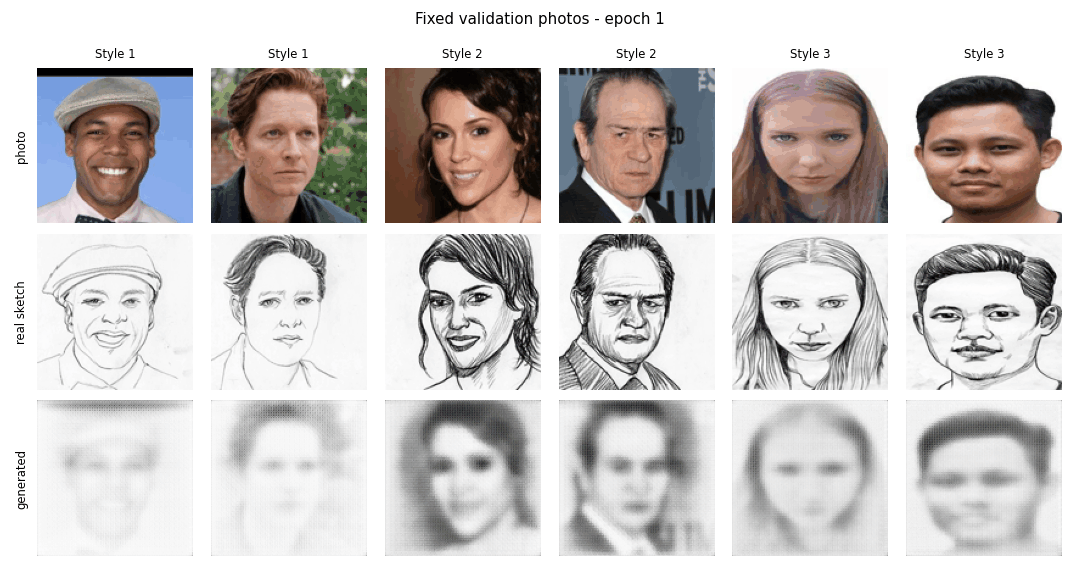
\includegraphics[width=0.32\textwidth]{task4_samples_epoch_001.png}}{}\hfill
\figif[0.32\textwidth]{task4_samples_mid.png}\hfill
\figif[0.32\textwidth]{task4_samples_last.png}
\caption{Generator development on the same fixed validation photographs: first, middle and final epoch.}\label{fig:t4evo}
\end{figure*}

\begin{figure*}[t]\centering
\figif[0.48\textwidth]{task4_style_swap_test.png}\hfill
\figif[0.5\textwidth]{task4_test_best_worst.png}
\caption{Left: the same test photograph rendered in all three styles (ground-truth style shown in column 2). Right: best and worst test samples by SSIM.}\label{fig:t4swap}
\end{figure*}

\textbf{Search outcome.} Ten six-epoch trials were run (5 pruned); the first trial used the pix2pix defaults. The best configuration uses $C{=}32$ base channels (10.6\,M generator parameters, 42\,MB ONNX), batch size 16, $\mathrm{lr}_G{=}4.2{\cdot}10^{-4}$, $\mathrm{lr}_D{=}2.3{\cdot}10^{-4}$, dropout 0.22, a 32-dimensional style embedding and $\lambda_{L1}{=}87.5$, close to the value of 100 commonly used in pix2pix. A slower discriminator than generator appears to be preferred because $D$ otherwise wins quickly on this small dataset (899 training pairs).

\textbf{Training dynamics.} Over 80 epochs (Fig.~\ref{fig:t4curves}) the discriminator's real loss fell from 0.88 to $\approx$0.6 and its fake loss from 0.70 to $\approx$0.37, while the generator's adversarial loss settled at 1.3--1.5. Neither network collapsed: $D$'s fake loss never approached zero, and the adversarial term stayed bounded. The L1 term fell from 0.30 to 0.175 and validation SSIM rose from 0.46 to $\approx$0.55. The fixed validation grids (Fig.~\ref{fig:t4evo}) show the generator moving from blurry face silhouettes to recognisable hair outlines, eyes and mouths.

\textbf{Test results.} On the 1,046 official test pairs the generator reaches L1 0.102, SSIM 0.549 and PSNR 16.1\,dB (Table~\ref{tab:gan}). Style~1 (light pencil, $n{=}619$) and Style~3 ($n{=}46$) are reproduced best (SSIM 0.59 and 0.67). Style~2 (dense dark hatching, $n{=}381$) is hardest (SSIM 0.46): its high-contrast strokes are drawn at artist-specific positions that a pixel-aligned model cannot predict, so the generator outputs an average shading that L1 and SSIM both penalise. Note also that the test split is strongly imbalanced across styles (619/381/46), unlike the balanced training split (303/298/298), so the overall figure is dominated by Styles~1 and~2.

\textbf{Is the style condition used?} Fig.~\ref{fig:t4swap} (left) renders the same test photograph in all three styles. Style~1 produces thin, light outlines; Style~2 adds dark shading in hair and around the eyes; Style~3 is in between. The embedding therefore changes the output substantially, as required, rather than acting only as an interface label. The worst test cases (Fig.~\ref{fig:t4swap}, right) are Style-2 sketches with heavy hatching, faces at unusual angles, and photos whose background has a colour similar to the hair.


%=====================================================================
\section{Experiment Tracking, Export and Deployment}
\textbf{Tracking.} Every Optuna trial is a nested MLflow run with its parameters and per-epoch metrics; final runs additionally log curves, sample grids, confusion matrices and result JSONs. Optuna studies are stored in SQLite so interrupted Kaggle/Colab sessions resume; every pipeline stage is skipped when its output already exists.

\textbf{ONNX.} All inference models (UDAE, classifier with softmax head, three specialists, the complete soft-MoE pipeline with outputs \texttt{output}, \texttt{weights}, \texttt{logits}, and the generator with an int64 \texttt{style} input) are exported at opset 17 with a dynamic batch axis and compared with PyTorch on random inputs (Table~\ref{tab:onnx}).

\inputif{onnx.tex}

\textbf{Application.} The interface was first designed in Google Stitch (Fig.~\ref{fig:stitch}) and then implemented in React with Tailwind CSS (Fig.~\ref{fig:app}). It contains the four required workspaces: \emph{Universal Restoration}, \emph{Hard-Routed Restoration}, \emph{Soft Mixture-of-Experts Restoration} and \emph{Face-to-Sketch Generator}, plus a system-status page. A user uploads an image (or a webcam capture for sketches) or selects a clean sample, applies a corruption at a chosen severity and seed, and sees the clean reference, input, output, PSNR/SSIM, inference time and the exact corruption parameters; the hard-routing view shows the four class probabilities, the predicted class and the executed expert (with an oracle/predicted toggle); the MoE view shows all four weights and the dominant contributor; results can be downloaded. The FastAPI backend validates type and size, decodes and resizes the image, applies the \emph{same} corruption module used during training (copied into the image at build time), runs ONNX Runtime and returns base64 images with routing and timing information. Endpoints: \texttt{/api/health}, \texttt{/api/restore/universal}, \texttt{/api/restore/hard}, \texttt{/api/restore/soft}, \texttt{/api/sketch}. Docker Compose (Fig.~\ref{fig:sys}) starts the backend, the nginx-served front end and an MLflow UI with \texttt{docker compose up --build}; the ONNX models are downloaded automatically from the GitHub release on first start.

\begin{figure}[t]\centering
\figif{arch_system.png}
\caption{Deployment architecture.}\label{fig:sys}
\end{figure}

\begin{figure}[t]\centering
\figif{stitch_design.png}
\caption{Original Google Stitch design of the application.}\label{fig:stitch}
\end{figure}

\begin{figure*}[t]\centering
\figif[0.49\textwidth]{app_hard.png}\hfill
\figif[0.49\textwidth]{app_soft.png}\\[4pt]
\figif[0.49\textwidth]{app_universal.png}\hfill
\figif[0.49\textwidth]{app_sketch.png}
\caption{Screenshots of the deployed application: hard routing, soft MoE, universal restoration and face-to-sketch workspaces.}\label{fig:app}
\end{figure*}

%=====================================================================
\section{Limitations}\label{sec:limits}
\begin{itemize}
\item \textbf{Compute.} All training ran on free Kaggle/Colab GPUs on the day of submission, so Optuna studies used 8--12 trials with short schedules (4--6 epochs per trial), which biases selection towards fast-converging configurations (e.g.\ the smallest bottleneck); larger searches and longer training would likely improve all results, particularly the GAN.
\item \textbf{Bottleneck vs.\ sharpness.} Without skip connections, fine textures (fur) must pass through an $8{\times}8$ code; outputs are smoother than the targets. This is the intended price of the autoencoder requirement.
\item \textbf{Inpainting.} Large occlusions require hallucinating content; L1/SSIM-trained models produce plausible but blurry fills. An adversarial or perceptual term would help.
\item \textbf{GAN evaluation.} Pixel metrics (L1/SSIM) do not fully capture sketch quality and bias the selection towards large $\lambda_{L1}$; FID/LPIPS were not computed for time reasons.
\item \textbf{Single corruptions.} Training never contains compound corruptions; the MoE gate then selects the most salient corruption instead of composing experts (Fig.~\ref{fig:t3dist}).
\end{itemize}

%=====================================================================
\section{Conclusion}
Under identical data and test conditions, the three restoration designs behave very differently. A single bottlenecked autoencoder removes impulse noise and fills holes, but it degrades every input to about 24\,dB, including clean and mildly blurred images. Hard routing with a 99.7\%-accurate classifier keeps clean images untouched and improves structural similarity, but it inherits the experts' fidelity ceiling, and its rare errors cost the most on clean images. The jointly trained soft MoE performed best (23.9\,dB / 0.786 SSIM on corrupted inputs, 46\,dB on clean ones) because, without any severity supervision, its gate learned to blend the identity branch with the expert in proportion to how strongly the image is corrupted. The main open problems are the bottleneck's fidelity ceiling and composing experts for compound corruptions. For face-to-sketch generation, a style-embedding pix2pix cGAN produces clearly style-dependent sketches (test SSIM 0.55), with dense-hatching Style~2 the hardest case. All models run in a single containerised application with verified ONNX inference and complete MLflow experiment records.


%=====================================================================
\appendices
\section{AI-Use Statement}
In line with the assignment policy, the following AI tools were used:
\begin{itemize}
\item \textbf{Claude (Anthropic), via the Claude desktop app}: used as a coding assistant to draft the training/evaluation code, the FastAPI backend, the React front end, the Docker configuration, the diagram script and an initial draft of this report from the assignment specification and from my design decisions.
\item \textbf{Google Stitch}: used, as required, to produce the initial UI design.
\end{itemize}
\textbf{Verification.} Every component was executed end-to-end: the whole pipeline (all four tasks) was first run in a reduced ``smoke'' configuration on CPU to catch shape, data and export errors; ONNX outputs were compared numerically with PyTorch (Table~\ref{tab:onnx}); the backend endpoints were exercised with valid and invalid uploads (e.g.\ non-image files return HTTP 415); the front end was built and checked in a browser against the running backend. Issues found and corrected during this process included: MLflow~3 refusing the file-based tracking store (fixed by an explicit opt-in so runs can be zipped and served offline), the need for an $\alpha$-independent Optuna objective, freezing expert batch-norm statistics during joint MoE training, and per-worker RNG seeding so that DataLoader workers do not generate identical corruptions. All reported numbers come from the logged runs, not from the assistant. I am responsible for the submitted work and can explain and modify any part of it.

\bibliographystyle{IEEEtran}
\begin{thebibliography}{99}
\bibitem{vincent2008} P.~Vincent, H.~Larochelle, Y.~Bengio and P.-A.~Manzagol, ``Extracting and composing robust features with denoising autoencoders,'' in \emph{Proc.\ ICML}, 2008, pp.~1096--1103.
\bibitem{mao2016} X.-J.~Mao, C.~Shen and Y.-B.~Yang, ``Image restoration using very deep convolutional encoder-decoder networks with symmetric skip connections,'' in \emph{Proc.\ NeurIPS}, 2016.
\bibitem{ronneberger2015} O.~Ronneberger, P.~Fischer and T.~Brox, ``U-Net: Convolutional networks for biomedical image segmentation,'' in \emph{Proc.\ MICCAI}, 2015, pp.~234--241.
\bibitem{zhao2017} H.~Zhao, O.~Gallo, I.~Frosio and J.~Kautz, ``Loss functions for image restoration with neural networks,'' \emph{IEEE Trans.\ Comput.\ Imaging}, vol.~3, no.~1, pp.~47--57, 2017.
\bibitem{wang2004} Z.~Wang, A.~C.~Bovik, H.~R.~Sheikh and E.~P.~Simoncelli, ``Image quality assessment: From error visibility to structural similarity,'' \emph{IEEE Trans.\ Image Process.}, vol.~13, no.~4, pp.~600--612, 2004.
\bibitem{zhang2017} K.~Zhang, W.~Zuo, Y.~Chen, D.~Meng and L.~Zhang, ``Beyond a Gaussian denoiser: Residual learning of deep CNN for image denoising,'' \emph{IEEE Trans.\ Image Process.}, vol.~26, no.~7, pp.~3142--3155, 2017.
\bibitem{li2022airnet} B.~Li, X.~Liu, P.~Hu, Z.~Wu, J.~Lv and X.~Peng, ``All-in-one image restoration for unknown corruption,'' in \emph{Proc.\ CVPR}, 2022, pp.~17452--17462.
\bibitem{potlapalli2023} V.~Potlapalli, S.~W.~Zamir, S.~Khan and F.~S.~Khan, ``PromptIR: Prompting for all-in-one blind image restoration,'' in \emph{Proc.\ NeurIPS}, 2023.
\bibitem{jacobs1991} R.~A.~Jacobs, M.~I.~Jordan, S.~J.~Nowlan and G.~E.~Hinton, ``Adaptive mixtures of local experts,'' \emph{Neural Computation}, vol.~3, no.~1, pp.~79--87, 1991.
\bibitem{shazeer2017} N.~Shazeer \emph{et al.}, ``Outrageously large neural networks: The sparsely-gated mixture-of-experts layer,'' in \emph{Proc.\ ICLR}, 2017.
\bibitem{fedus2022} W.~Fedus, B.~Zoph and N.~Shazeer, ``Switch Transformers: Scaling to trillion parameter models with simple and efficient sparsity,'' \emph{JMLR}, vol.~23, no.~120, pp.~1--39, 2022.
\bibitem{isola2017} P.~Isola, J.-Y.~Zhu, T.~Zhou and A.~A.~Efros, ``Image-to-image translation with conditional adversarial networks,'' in \emph{Proc.\ CVPR}, 2017, pp.~1125--1134.
\bibitem{mirza2014} M.~Mirza and S.~Osindero, ``Conditional generative adversarial nets,'' arXiv:1411.1784, 2014.
\bibitem{fan2022fs2k} D.-P.~Fan, Z.~Huang, P.~Zheng, H.~Liu, X.~Qin and L.~Van~Gool, ``Facial-sketch synthesis: A new challenge,'' \emph{Machine Intelligence Research}, vol.~19, pp.~257--287, 2022.
\bibitem{akiba2019} T.~Akiba, S.~Sano, T.~Yanase, T.~Ohta and M.~Koyama, ``Optuna: A next-generation hyperparameter optimization framework,'' in \emph{Proc.\ KDD}, 2019, pp.~2623--2631.
\bibitem{zaharia2018} M.~Zaharia \emph{et al.}, ``Accelerating the machine learning lifecycle with MLflow,'' \emph{IEEE Data Eng.\ Bull.}, vol.~41, no.~4, pp.~39--45, 2018.
\end{thebibliography}

\end{document}
